% Options for packages loaded elsewhere
\PassOptionsToPackage{unicode}{hyperref}
\PassOptionsToPackage{hyphens}{url}
%
\documentclass[
  a4paper,
]{article}
\usepackage{amsmath,amssymb}
\usepackage{iftex}
\ifPDFTeX
  \usepackage[T1]{fontenc}
  \usepackage[utf8]{inputenc}
  \usepackage{textcomp} % provide euro and other symbols
\else % if luatex or xetex
  \usepackage{unicode-math} % this also loads fontspec
  \defaultfontfeatures{Scale=MatchLowercase}
  \defaultfontfeatures[\rmfamily]{Ligatures=TeX,Scale=1}
\fi
\usepackage{lmodern}
\ifPDFTeX\else
  % xetex/luatex font selection
  \setmainfont[]{Helvetica}
\fi
% Use upquote if available, for straight quotes in verbatim environments
\IfFileExists{upquote.sty}{\usepackage{upquote}}{}
\IfFileExists{microtype.sty}{% use microtype if available
  \usepackage[]{microtype}
  \UseMicrotypeSet[protrusion]{basicmath} % disable protrusion for tt fonts
}{}
\makeatletter
\@ifundefined{KOMAClassName}{% if non-KOMA class
  \IfFileExists{parskip.sty}{%
    \usepackage{parskip}
  }{% else
    \setlength{\parindent}{0pt}
    \setlength{\parskip}{6pt plus 2pt minus 1pt}}
}{% if KOMA class
  \KOMAoptions{parskip=half}}
\makeatother
\usepackage{xcolor}
\usepackage[margin=0.75in]{geometry}
\usepackage{graphicx}
\makeatletter
\def\maxwidth{\ifdim\Gin@nat@width>\linewidth\linewidth\else\Gin@nat@width\fi}
\def\maxheight{\ifdim\Gin@nat@height>\textheight\textheight\else\Gin@nat@height\fi}
\makeatother
% Scale images if necessary, so that they will not overflow the page
% margins by default, and it is still possible to overwrite the defaults
% using explicit options in \includegraphics[width, height, ...]{}
\setkeys{Gin}{width=\maxwidth,height=\maxheight,keepaspectratio}
% Set default figure placement to htbp
\makeatletter
\def\fps@figure{htbp}
\makeatother
\setlength{\emergencystretch}{3em} % prevent overfull lines
\providecommand{\tightlist}{%
  \setlength{\itemsep}{0pt}\setlength{\parskip}{0pt}}
\setcounter{secnumdepth}{-\maxdimen} % remove section numbering
\usepackage{titling}
\pretitle{\begin{flushleft}}
\posttitle{\end{flushleft}}
\usepackage{booktabs}
\usepackage{longtable}
\usepackage{float}
\floatplacement{figure}{H}
\usepackage{colortbl}
\usepackage{pdflscape}
\usepackage{tabu}
\usepackage{makecell}
\usepackage{xcolor}
\usepackage{soul}
\usepackage{caption}
\usepackage[singlelinecheck=false]{caption}
\usepackage[font={small,bf}]{caption}
\usepackage{multirow}
\usepackage{array}
\usepackage{lscape}
\newcommand{\blandscape}{\begin{landscape}}
\newcommand{\elandscape}{\end{landscape}}
\usepackage[dvipsnames]{xcolor}
\renewcommand{\footnotesize}{\tiny}
\usepackage{booktabs}
\usepackage{longtable}
\usepackage{array}
\usepackage{multirow}
\usepackage{wrapfig}
\usepackage{float}
\usepackage{colortbl}
\usepackage{pdflscape}
\usepackage{tabu}
\usepackage{threeparttable}
\usepackage{threeparttablex}
\usepackage[normalem]{ulem}
\usepackage{makecell}
\usepackage{xcolor}
\ifLuaTeX
  \usepackage{selnolig}  % disable illegal ligatures
\fi
\usepackage{bookmark}
\IfFileExists{xurl.sty}{\usepackage{xurl}}{} % add URL line breaks if available
\urlstyle{same}
\hypersetup{
  hidelinks,
  pdfcreator={LaTeX via pandoc}}

\title{\vspace{-1.5cm} \begin{LARGE} WGS Quality Control Report \end{LARGE}}
\author{}
\date{\vspace{-2.5em}}

\begin{document}
\maketitle

\normalsize Batch Name: 2024-08-02

\normalsize Experiment Name: 24ARS\_SALM\_EMR\_LG73M

\fontsize{7}{8}
\selectfont
\captionsetup[table]{labelformat=empty}
\renewcommand{\arraystretch}{1.2}

\begin{longtable}[t]{>{\centering\arraybackslash}p{1cm}>{\centering\arraybackslash}p{2cm}>{\centering\arraybackslash}p{1.5cm}>{\centering\arraybackslash}p{5.25cm}>{\centering\arraybackslash}p{5.25cm}}
\toprule
\multicolumn{1}{>{\centering\arraybackslash}p{1cm}}{\cellcolor[HTML]{D4D4D4}{\textbf{Isolate No.}}} & \multicolumn{1}{>{\centering\arraybackslash}p{2cm}}{\cellcolor[HTML]{D4D4D4}{\textbf{Sample ID}}} & \multicolumn{1}{>{\centering\arraybackslash}p{1.5cm}}{\cellcolor[HTML]{D4D4D4}{\textbf{Description}}} & \multicolumn{1}{>{\centering\arraybackslash}p{5.25cm}}{\cellcolor[HTML]{D4D4D4}{\textbf{ARSRL}}} & \multicolumn{1}{>{\centering\arraybackslash}p{5.25cm}}{\cellcolor[HTML]{D4D4D4}{\textbf{WGS}}}\\
\midrule
\cellcolor[HTML]{FFA77F}{1} & \cellcolor[HTML]{FFA77F}{24ARS\_DMC0037} & \cellcolor[HTML]{FFA77F}{NGO50} & \cellcolor[HTML]{FFA77F}{*Neisseria gonorrhoeae} & \cellcolor[HTML]{FFA77F}{Neisseria gonorrhoeae}\\
2 & 24ARS\_JLM0047 & SAL105 & Salmonella Typhi & Salmonella typhi\\
3 & 24ARS\_JLM0082 & SAL106 & Salmonella species & Salmonella enterica\\
\cellcolor[HTML]{FFA77F}{4} & \cellcolor[HTML]{FFA77F}{24ARS\_MAR0001} & \cellcolor[HTML]{FFA77F}{NGO51} & \cellcolor[HTML]{FFA77F}{Neisseria gonorrhoeae} & \cellcolor[HTML]{FFA77F}{Neisseria gonorrhoeae}\\
5 & 24ARS\_MAR0067 & SAL107 & Salmonella species & Salmonella enterica\\
\addlinespace
\cellcolor[HTML]{FFA77F}{6} & \cellcolor[HTML]{FFA77F}{24ARS\_MAR0073} & \cellcolor[HTML]{FFA77F}{NGO52} & \cellcolor[HTML]{FFA77F}{Neisseria gonorrhoeae} & \cellcolor[HTML]{FFA77F}{Neisseria gonorrhoeae}\\
\cellcolor[HTML]{FFA77F}{7} & \cellcolor[HTML]{FFA77F}{24ARS\_MAR0074} & \cellcolor[HTML]{FFA77F}{NGO53} & \cellcolor[HTML]{FFA77F}{Neisseria gonorrhoeae} & \cellcolor[HTML]{FFA77F}{Neisseria gonorrhoeae}\\
8 & 24ARS\_SLH0029 & SAL110 & Salmonella species & Salmonella enterica\\
9 & 24ARS\_SLH0035 & SAL111 & Salmonella species & Salmonella enterica\\
10 & 24ARS\_SLH0036 & NGO54 & *Neisseria gonorrhoeae & Neisseria gonorrhoeae\\
\addlinespace
11 & 24ARS\_SLH0047 & SAL112 & Salmonella species & Salmonella enterica\\
12 & 24ARS\_SLH0063 & SAL113 & Salmonella species & Salmonella enterica\\
13 & 24ARS\_STU0025 & SAL115 & Salmonella species & Salmonella enterica\\
\cellcolor[HTML]{FFA77F}{14} & \cellcolor[HTML]{FFA77F}{24ARS\_STU0034} & \cellcolor[HTML]{FFA77F}{SAL116} & \cellcolor[HTML]{FFA77F}{Salmonella species} & \cellcolor[HTML]{FFA77F}{Salmonella enterica}\\
\cellcolor[HTML]{FD7979}{15} & \cellcolor[HTML]{FD7979}{24ARS\_VSM0001} & \cellcolor[HTML]{FD7979}{NGO55} & \cellcolor[HTML]{FD7979}{Neisseria gonorrhoeae} & \cellcolor[HTML]{FD7979}{Neisseria gonorrhoeae}\\
\addlinespace
\cellcolor[HTML]{FFA77F}{16} & \cellcolor[HTML]{FFA77F}{24ARS\_VSM0056} & \cellcolor[HTML]{FFA77F}{SAL118} & \cellcolor[HTML]{FFA77F}{Salmonella species} & \cellcolor[HTML]{FFA77F}{Salmonella enterica}\\
17 & 24ARS\_VSM0059 & SAL121 & Salmonella species & Salmonella enterica\\
\cellcolor[HTML]{FD7979}{18} & \cellcolor[HTML]{FD7979}{24ARS\_VSM0093} & \cellcolor[HTML]{FD7979}{NGO56} & \cellcolor[HTML]{FD7979}{Neisseria gonorrhoeae} & \cellcolor[HTML]{FD7979}{Neisseria gonorrhoeae}\\
19 & 24ARS\_VSM0200 & SAL124 & Salmonella species & Salmonella enterica\\
20 & 24ARS\_ZMC0010 & SAL125 & Salmonella Typhi & Salmonella typhi\\
\addlinespace
21 & 24ARS\_ZMC0013 & SAL126 & Salmonella Typhi & Salmonella typhi\\
22 & 24ARS\_ZMC0014 & SAL127 & Salmonella Typhi & Salmonella typhi\\
\bottomrule
\multicolumn{5}{l}{\rule{0pt}{1em}\textit{Legend:} PASS   |   \colorbox{Peach}{WARNING}   |   \colorbox{Salmon}{FAILURE}   |   \textcolor{Blue}{EXCEEDS THRESHOLD METRIC/S}   |   (x) - NON-CONCORDANT   |}\\
\end{longtable}

\fontsize{7}{8}
\selectfont
\captionsetup[table]{labelformat=empty}
\renewcommand{\arraystretch}{1.2}

\(\\\)

\fontsize{7}{8}
\selectfont
\captionsetup[table]{labelformat=empty}
\renewcommand{\arraystretch}{1.2}

\begin{ThreePartTable}
\begin{TableNotes}[para]
\item \textit{Legend:} 
\item PASS
\item   |  
\item \colorbox{Peach}{WARNING}
\item   |  
\item \colorbox{Salmon}{FAILURE}
\item   |  
\item \textcolor{Blue}{EXCEEDS THRESHOLD METRIC/S}
\item   |  
\end{TableNotes}
\begin{longtable}[t]{>{\centering\arraybackslash}p{1cm}>{\centering\arraybackslash}p{3cm}>{\centering\arraybackslash}p{2cm}>{\centering\arraybackslash}p{2cm}>{\centering\arraybackslash}p{2cm}>{\centering\arraybackslash}p{2cm}>{\centering\arraybackslash}p{2cm}}
\toprule
\multicolumn{1}{>{\centering\arraybackslash}p{1cm}}{\cellcolor[HTML]{D4D4D4}{\textbf{Isolate No.}}} & \multicolumn{1}{>{\centering\arraybackslash}p{3cm}}{\cellcolor[HTML]{D4D4D4}{\textbf{Sample ID}}} & \multicolumn{1}{>{\centering\arraybackslash}p{2cm}}{\cellcolor[HTML]{D4D4D4}{\textbf{Contamination}}} & \multicolumn{1}{>{\centering\arraybackslash}p{2cm}}{\cellcolor[HTML]{D4D4D4}{\textbf{Contigs}}} & \multicolumn{1}{>{\centering\arraybackslash}p{2cm}}{\cellcolor[HTML]{D4D4D4}{\textbf{GC Percent}}} & \multicolumn{1}{>{\centering\arraybackslash}p{2cm}}{\cellcolor[HTML]{D4D4D4}{\textbf{N50}}} & \multicolumn{1}{>{\centering\arraybackslash}p{2cm}}{\cellcolor[HTML]{D4D4D4}{\textbf{Total Length}}}\\
\midrule
\cellcolor[HTML]{FFA77F}{1} & \cellcolor[HTML]{FFA77F}{24ARS\_DMC0037} & \cellcolor[HTML]{FFA77F}{\textcolor{black}{0.00}} & \cellcolor[HTML]{FFA77F}{\textcolor{black}{86}} & \cellcolor[HTML]{FFA77F}{52.50} & \cellcolor[HTML]{FFA77F}{\textcolor{blue}{48608}} & \cellcolor[HTML]{FFA77F}{2125667}\\
2 & 24ARS\_JLM0047 & \textcolor{black}{0.00} & \textcolor{black}{52} & 52.06 & \textcolor{black}{204329} & 4717836\\
3 & 24ARS\_JLM0082 & \textcolor{black}{0.00} & \textcolor{black}{25} & 52.12 & \textcolor{black}{489949} & 4730692\\
\cellcolor[HTML]{FFA77F}{4} & \cellcolor[HTML]{FFA77F}{24ARS\_MAR0001} & \cellcolor[HTML]{FFA77F}{\textcolor{black}{0.00}} & \cellcolor[HTML]{FFA77F}{\textcolor{black}{95}} & \cellcolor[HTML]{FFA77F}{52.54} & \cellcolor[HTML]{FFA77F}{\textcolor{blue}{47364}} & \cellcolor[HTML]{FFA77F}{2106255}\\
5 & 24ARS\_MAR0067 & \textcolor{black}{0.00} & \textcolor{black}{23} & 52.13 & \textcolor{black}{490374} & 4702134\\
\addlinespace
\cellcolor[HTML]{FFA77F}{6} & \cellcolor[HTML]{FFA77F}{24ARS\_MAR0073} & \cellcolor[HTML]{FFA77F}{\textcolor{black}{0.00}} & \cellcolor[HTML]{FFA77F}{\textcolor{black}{88}} & \cellcolor[HTML]{FFA77F}{52.41} & \cellcolor[HTML]{FFA77F}{\textcolor{blue}{48589}} & \cellcolor[HTML]{FFA77F}{2133215}\\
\cellcolor[HTML]{FFA77F}{7} & \cellcolor[HTML]{FFA77F}{24ARS\_MAR0074} & \cellcolor[HTML]{FFA77F}{\textcolor{black}{0.00}} & \cellcolor[HTML]{FFA77F}{\textcolor{black}{96}} & \cellcolor[HTML]{FFA77F}{52.46} & \cellcolor[HTML]{FFA77F}{\textcolor{blue}{49562}} & \cellcolor[HTML]{FFA77F}{2120328}\\
8 & 24ARS\_SLH0029 & \textcolor{black}{0.00} & \textcolor{black}{57} & 52.13 & \textcolor{black}{333142} & 4977595\\
9 & 24ARS\_SLH0035 & \textcolor{black}{0.00} & \textcolor{black}{25} & 52.13 & \textcolor{black}{490573} & 4701900\\
10 & 24ARS\_SLH0036 & \textcolor{black}{0.00} & \textcolor{black}{86} & 52.55 & \textcolor{black}{50737} & 2122346\\
\addlinespace
11 & 24ARS\_SLH0047 & \textcolor{black}{0.00} & \textcolor{black}{38} & 52.21 & \textcolor{black}{376618} & 4872581\\
12 & 24ARS\_SLH0063 & \textcolor{black}{0.00} & \textcolor{black}{23} & 52.13 & \textcolor{black}{490374} & 4701747\\
13 & 24ARS\_STU0025 & \textcolor{black}{0.00} & \textcolor{black}{33} & 52.17 & \textcolor{black}{741543} & 4736398\\
\cellcolor[HTML]{FFA77F}{14} & \cellcolor[HTML]{FFA77F}{* 24ARS\_STU0034} & \cellcolor[HTML]{FFA77F}{\textcolor{black}{0.00}} & \cellcolor[HTML]{FFA77F}{\textcolor{black}{27}} & \cellcolor[HTML]{FFA77F}{52.03} & \cellcolor[HTML]{FFA77F}{\textcolor{black}{490410}} & \cellcolor[HTML]{FFA77F}{4750129}\\
\cellcolor[HTML]{FD7979}{15} & \cellcolor[HTML]{FD7979}{24ARS\_VSM0001} & \cellcolor[HTML]{FD7979}{\textcolor{blue}{16.33}} & \cellcolor[HTML]{FD7979}{\textcolor{black}{116}} & \cellcolor[HTML]{FD7979}{52.48} & \cellcolor[HTML]{FD7979}{\textcolor{blue}{47291}} & \cellcolor[HTML]{FD7979}{2130195}\\
\addlinespace
\cellcolor[HTML]{FFA77F}{16} & \cellcolor[HTML]{FFA77F}{* 24ARS\_VSM0056} & \cellcolor[HTML]{FFA77F}{\textcolor{black}{0.00}} & \cellcolor[HTML]{FFA77F}{\textcolor{black}{24}} & \cellcolor[HTML]{FFA77F}{52.10} & \cellcolor[HTML]{FFA77F}{\textcolor{black}{489948}} & \cellcolor[HTML]{FFA77F}{4724471}\\
17 & 24ARS\_VSM0059 & \textcolor{black}{0.00} & \textcolor{black}{24} & 52.13 & \textcolor{black}{489948} & 4699372\\
\cellcolor[HTML]{FD7979}{18} & \cellcolor[HTML]{FD7979}{24ARS\_VSM0093} & \cellcolor[HTML]{FD7979}{\textcolor{blue}{9.91}} & \cellcolor[HTML]{FD7979}{\textcolor{black}{107}} & \cellcolor[HTML]{FD7979}{52.48} & \cellcolor[HTML]{FD7979}{\textcolor{blue}{48884}} & \cellcolor[HTML]{FD7979}{2129502}\\
19 & 24ARS\_VSM0200 & \textcolor{black}{0.00} & \textcolor{black}{52} & 52.17 & \textcolor{black}{301432} & 4907981\\
20 & 24ARS\_ZMC0010 & \textcolor{black}{0.00} & \textcolor{black}{55} & 52.05 & \textcolor{black}{204322} & 4721525\\
\addlinespace
21 & 24ARS\_ZMC0013 & \textcolor{black}{0.00} & \textcolor{black}{59} & 52.01 & \textcolor{black}{204322} & 4733565\\
22 & 24ARS\_ZMC0014 & \textcolor{black}{0.00} & \textcolor{black}{55} & 52.08 & \textcolor{black}{204320} & 4705524\\
\bottomrule
\multicolumn{7}{l}{\rule{0pt}{1em}\textit{Note: } *Isolates were tagged with warning due to uncertain results of species identification using bactinspector.}\\
\insertTableNotes
\end{longtable}
\end{ThreePartTable}

\fontsize{7}{8}
\selectfont
\captionsetup[table]{labelformat=empty}
\renewcommand{\arraystretch}{1.2}

\begin{longtable}[t]{>{\centering\arraybackslash}p{2cm}>{\raggedright\arraybackslash}p{3cm}>{\centering\arraybackslash}p{11cm}}
\toprule
\multicolumn{3}{l}{\textbf{With Warning/s}} \\
\cmidrule(l{3pt}r{3pt}){1-3}
\multicolumn{1}{>{\centering\arraybackslash}p{2cm}}{\cellcolor[HTML]{D4D4D4}{\textbf{Isolate No.}}} & \multicolumn{1}{>{\centering\arraybackslash}p{3cm}}{\cellcolor[HTML]{D4D4D4}{\textbf{Sample ID}}} & \multicolumn{1}{>{\centering\arraybackslash}p{11cm}}{\cellcolor[HTML]{D4D4D4}{\textbf{Value with warning/s}}}\\
\midrule
\cellcolor{gray!10}{1} & \cellcolor{gray!10}{24ARS\_DMC0037} & \cellcolor{gray!10}{fastqc.1.Per.sequence.GC.content.metric\_value, fastqc.1.Sequence.Duplication.Levels.metric\_value, fastqc.1.Sequence.Length.Distribution.metric\_value, fastqc.2.Per.sequence.GC.content.metric\_value, fastqc.2.Sequence.Duplication.Levels.metric\_value, fastqc.2.Sequence.Length.Distribution.metric\_value}\\
4 & 24ARS\_MAR0001 & fastqc.1.Per.sequence.GC.content.metric\_value, fastqc.1.Sequence.Duplication.Levels.metric\_value, fastqc.1.Sequence.Length.Distribution.metric\_value, fastqc.2.Per.sequence.GC.content.metric\_value, fastqc.2.Sequence.Duplication.Levels.metric\_value, fastqc.2.Sequence.Length.Distribution.metric\_value\\
\cellcolor{gray!10}{6} & \cellcolor{gray!10}{24ARS\_MAR0073} & \cellcolor{gray!10}{fastqc.1.Per.sequence.GC.content.metric\_value, fastqc.1.Sequence.Duplication.Levels.metric\_value, fastqc.1.Sequence.Length.Distribution.metric\_value, fastqc.2.Per.sequence.GC.content.metric\_value, fastqc.2.Sequence.Duplication.Levels.metric\_value, fastqc.2.Sequence.Length.Distribution.metric\_value}\\
7 & 24ARS\_MAR0074 & fastqc.1.Per.sequence.GC.content.metric\_value, fastqc.1.Sequence.Length.Distribution.metric\_value, fastqc.2.Per.sequence.GC.content.metric\_value, fastqc.2.Sequence.Length.Distribution.metric\_value\\
\cellcolor{gray!10}{14} & \cellcolor{gray!10}{24ARS\_STU0034} & \cellcolor{gray!10}{fastqc.1.Per.sequence.GC.content.metric\_value, fastqc.1.Sequence.Length.Distribution.metric\_value, fastqc.2.Per.sequence.GC.content.metric\_value, fastqc.2.Sequence.Length.Distribution.metric\_value}\\
\addlinespace
16 & 24ARS\_VSM0056 & fastqc.1.Per.sequence.GC.content.metric\_value, fastqc.1.Sequence.Length.Distribution.metric\_value, fastqc.2.Per.sequence.GC.content.metric\_value, fastqc.2.Sequence.Length.Distribution.metric\_value\\
\bottomrule
\end{longtable}

\begin{longtable}[l]{cccccc}
\toprule
\multicolumn{6}{l}{\textbf{List of samples above/below QC threshold metrics}} \\
\cmidrule(l{3pt}r{3pt}){1-6}
\cellcolor[HTML]{D4D4D4}{\textbf{Sample ID}} & \cellcolor[HTML]{D4D4D4}{\textbf{Result}} & \cellcolor[HTML]{D4D4D4}{\textbf{Contamination}} & \cellcolor[HTML]{D4D4D4}{\textbf{Contigs}} & \cellcolor[HTML]{D4D4D4}{\textbf{N50}} & \cellcolor[HTML]{D4D4D4}{\textbf{Total Length}}\\
\midrule
24ARS\_VSM0001 & FAILURE & FAILURE & 116 & 47291 & 2130195\\
24ARS\_VSM0093 & FAILURE & FAILURE & 107 & 48884 & 2129502\\
\bottomrule
\end{longtable}

\fontsize{7}{8}
\selectfont
\captionsetup[table]{labelformat=empty}
\renewcommand{\arraystretch}{1.2}

\begin{longtable}[l]{>{\raggedright\arraybackslash}p{8cm}c}
\toprule
\cellcolor[HTML]{D4D4D4}{\textbf{WGS\_ID}} & \cellcolor[HTML]{D4D4D4}{\textbf{Number}}\\
\midrule
Salmonella enterica & 11\\
Neisseria gonorrhoeae & 7\\
Salmonella typhi & 4\\
\bottomrule
\end{longtable}

\begin{itemize}
\item
  \(\color{red}3\) distinct species were identified among
  \(\color{red}22\) isolates.
\item
  \(\color{red}63.64\) \% (n=14) of the isolates passed the QC, while
  \(\color{red}27.27\) \% (n=6) were tagged with warning.
\item
  Concordance between ARSRL and WGS species report was
  \(\color{red}100.00\) \%. \(\\\)
\end{itemize}

\subsubsection{GRAPHS}\label{graphs}

\fontsize{7}{8}
\selectfont
\captionsetup[table]{labelformat=empty}
\renewcommand{\arraystretch}{1.2}

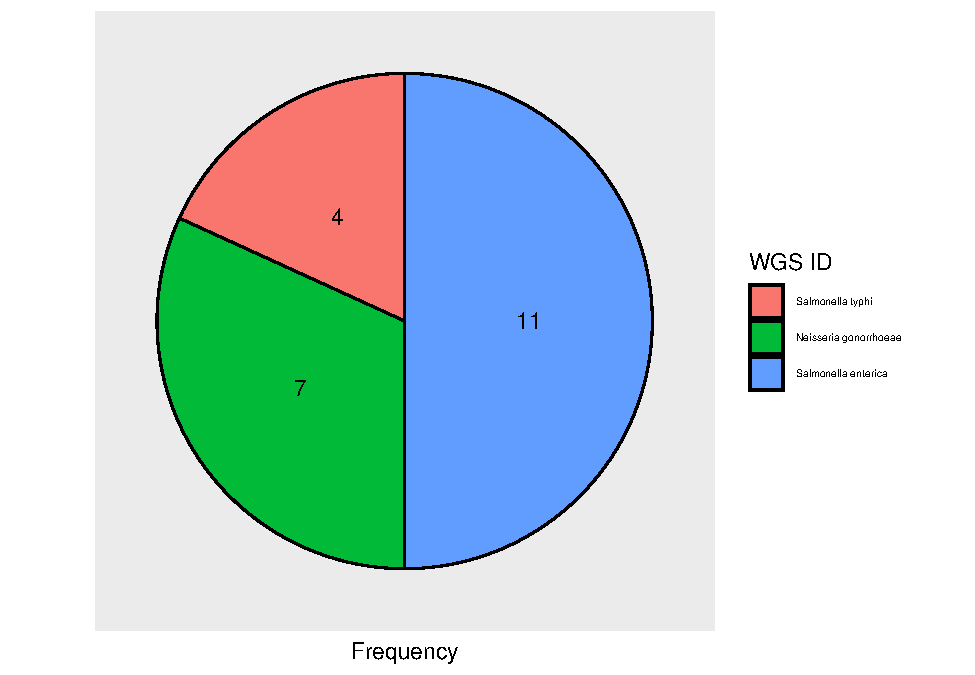
\includegraphics{qualifyr_report_2024-08-02_files/figure-latex/pie_chart-1.pdf}

\subsubsection{Result Classification}\label{result-classification}

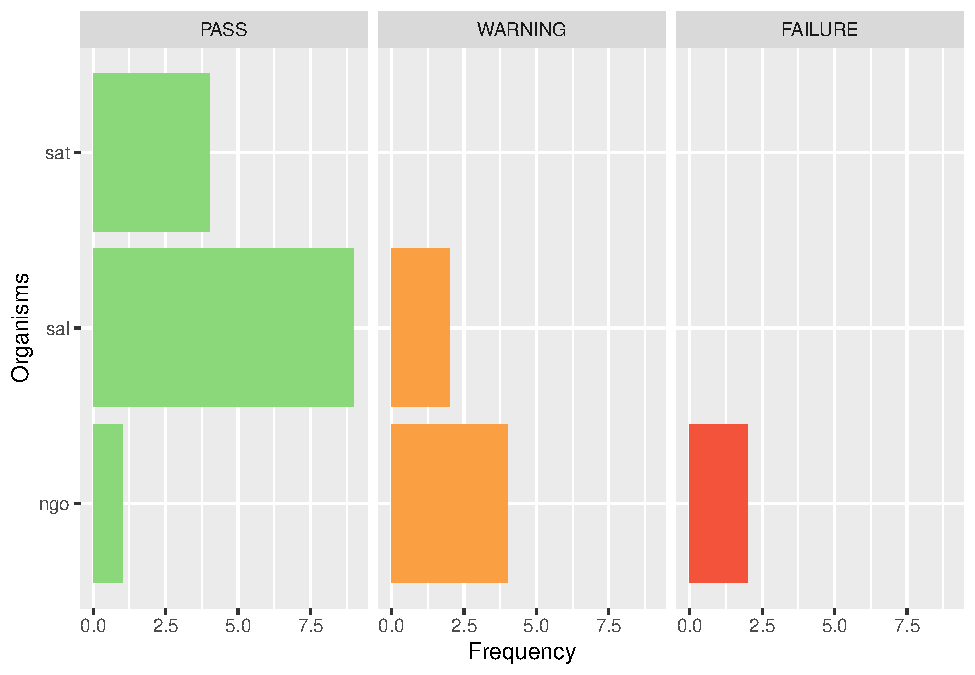
\includegraphics{qualifyr_report_2024-08-02_files/figure-latex/organism results-1.pdf}

\subsubsection{Number of contigs}\label{number-of-contigs}

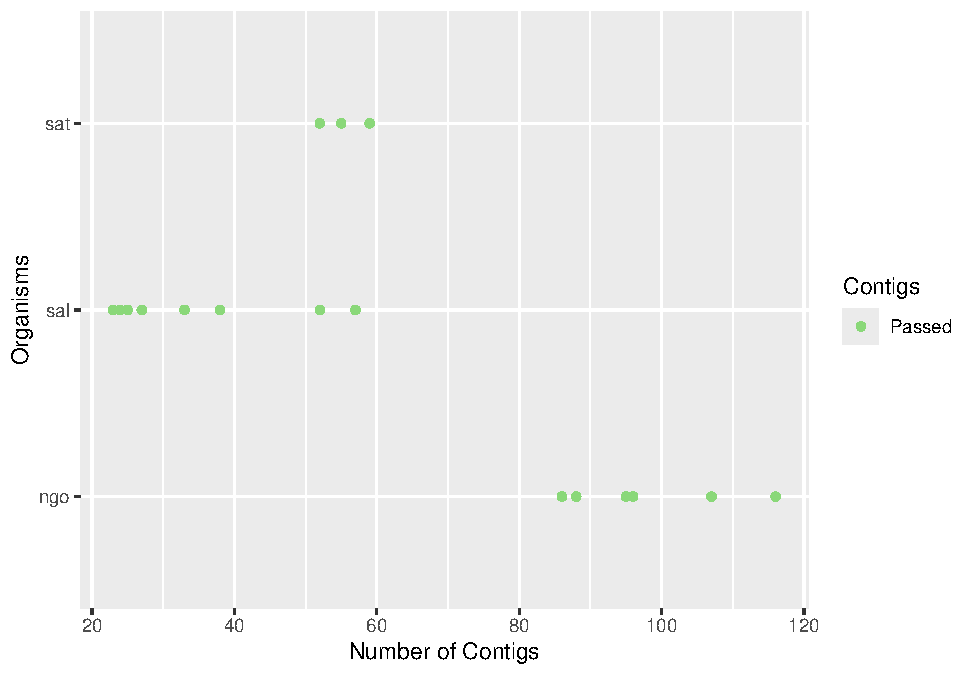
\includegraphics{qualifyr_report_2024-08-02_files/figure-latex/unnamed-chunk-1-1.pdf}

\subsubsection{N50 Value}\label{n50-value}

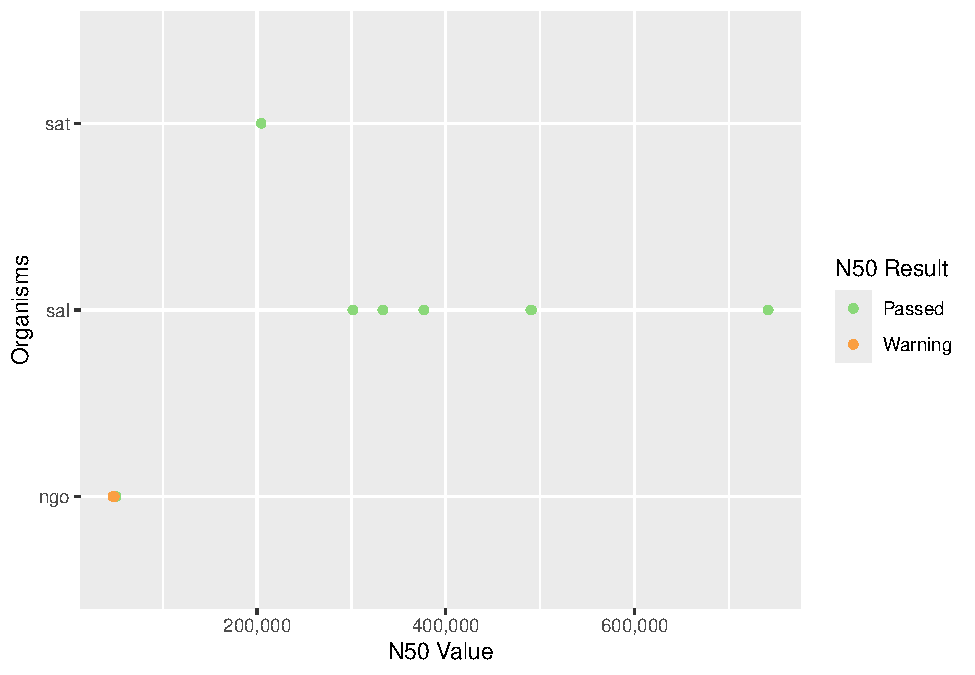
\includegraphics{qualifyr_report_2024-08-02_files/figure-latex/n50_result -1.pdf}

\subsubsection{Total Length}\label{total-length}

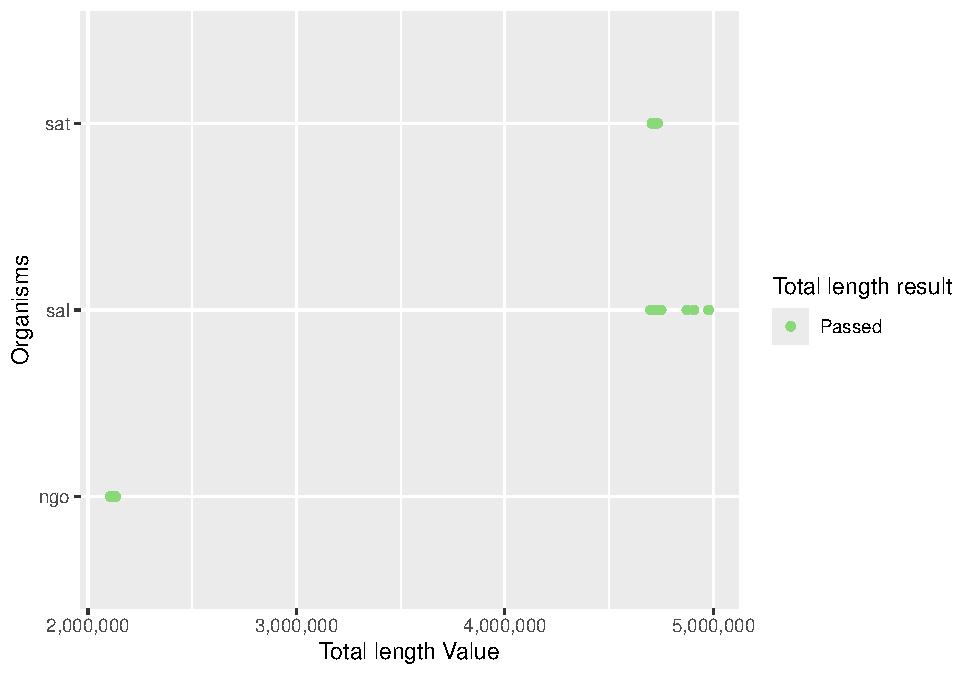
\includegraphics{qualifyr_report_2024-08-02_files/figure-latex/length_result -1.pdf}

\(\\\)

\subsubsection{RECOMMENDATION:}\label{recommendation}

\begin{longtable}[l]{>{\centering\arraybackslash}p{6cm}>{\centering\arraybackslash}p{4cm}>{\centering\arraybackslash}p{6cm}}
\toprule
\cellcolor[HTML]{D4D4D4}{\textbf{Sample ID}} & \cellcolor[HTML]{D4D4D4}{\textbf{Action}} & \cellcolor[HTML]{D4D4D4}{\textbf{Reason}}\\
\midrule
24ARS\_VSM0001 & Repeat testing & QC failure (high contigs \& N50 value)\\
24ARS\_VSM0093 & Repeat testing & QC failure (high contigs \& N50 value)\\
\bottomrule
\end{longtable}

\subsubsection{MLST RESULTS}\label{mlst-results}

\begin{longtable}[l]{>{\centering\arraybackslash}p{3cm}>{\centering\arraybackslash}p{3cm}>{\centering\arraybackslash}p{1cm}>{\centering\arraybackslash}p{1cm}>{\centering\arraybackslash}p{1cm}>{\centering\arraybackslash}p{1cm}>{\centering\arraybackslash}p{1cm}>{\centering\arraybackslash}p{1cm}>{\centering\arraybackslash}p{1cm}c}
\toprule
\cellcolor[HTML]{D4D4D4}{\textbf{sample\_id}} & \cellcolor[HTML]{D4D4D4}{\textbf{species}} & \cellcolor[HTML]{D4D4D4}{\textbf{MLST}} & \cellcolor[HTML]{D4D4D4}{\textbf{aroC.5.638.}} & \cellcolor[HTML]{D4D4D4}{\textbf{adk}} & \cellcolor[HTML]{D4D4D4}{\textbf{aroE}} & \cellcolor[HTML]{D4D4D4}{\textbf{fumC}} & \cellcolor[HTML]{D4D4D4}{\textbf{gdh}} & \cellcolor[HTML]{D4D4D4}{\textbf{pdhC}} & \cellcolor[HTML]{D4D4D4}{\textbf{pgm}}\\
\midrule
24ARS\_DMC0037 & Neisseria gonorrhoeae & 10316 & abcZ(59) & 39 & 67 & 157 & 149 & 71 & 65\\
24ARS\_MAR0001 & Neisseria gonorrhoeae & - & abcZ(59) & 39 & 67 & 156 & 149 & 530 & 65\\
24ARS\_MAR0073 & Neisseria gonorrhoeae & 8776 & abcZ(59) & 39 & 67 & 157 & 148 & 71 & 133\\
24ARS\_MAR0074 & Neisseria gonorrhoeae & 11249 & abcZ(59) & 39 & 67 & 157 & 148 & 71 & 65\\
24ARS\_SLH0036 & Neisseria gonorrhoeae & 1587 & abcZ(59) & 39 & 67 & 78 & 148 & 153 & 133\\
\addlinespace
24ARS\_VSM0001 & Neisseria gonorrhoeae & 7363 & abcZ(59) & 39 & 67 & 78 & 148 & 153 & 65\\
24ARS\_VSM0093 & Neisseria gonorrhoeae & 7363 & abcZ(59) & 39 & 67 & 78 & 148 & 153 & 65\\
\bottomrule
\multicolumn{10}{l}{\rule{0pt}{1em}\textit{Legend: } (-) Not identified}\\
\end{longtable}

\begin{longtable}[l]{>{\centering\arraybackslash}p{3cm}>{\centering\arraybackslash}p{3cm}>{\centering\arraybackslash}p{1cm}>{\centering\arraybackslash}p{1cm}>{\centering\arraybackslash}p{1cm}>{\centering\arraybackslash}p{1cm}>{\centering\arraybackslash}p{1cm}>{\centering\arraybackslash}p{1cm}>{\centering\arraybackslash}p{1cm}c}
\toprule
\cellcolor[HTML]{D4D4D4}{\textbf{sample\_id}} & \cellcolor[HTML]{D4D4D4}{\textbf{species}} & \cellcolor[HTML]{D4D4D4}{\textbf{MLST}} & \cellcolor[HTML]{D4D4D4}{\textbf{aroC.5.638.}} & \cellcolor[HTML]{D4D4D4}{\textbf{adk}} & \cellcolor[HTML]{D4D4D4}{\textbf{aroE}} & \cellcolor[HTML]{D4D4D4}{\textbf{fumC}} & \cellcolor[HTML]{D4D4D4}{\textbf{gdh}} & \cellcolor[HTML]{D4D4D4}{\textbf{pdhC}} & \cellcolor[HTML]{D4D4D4}{\textbf{pgm}}\\
\midrule
24ARS\_JLM0047 & Salmonella typhi & 1 & aroC(1) & 1 & 1 & 1 & 1 & 1 & 5\\
24ARS\_ZMC0010 & Salmonella typhi & 2 & aroC(1) & 1 & 2 & 1 & 1 & 1 & 5\\
24ARS\_ZMC0013 & Salmonella typhi & 2 & aroC(1) & 1 & 2 & 1 & 1 & 1 & 5\\
24ARS\_ZMC0014 & Salmonella typhi & 1 & aroC(1) & 1 & 1 & 1 & 1 & 1 & 5\\
\bottomrule
\multicolumn{10}{l}{\rule{0pt}{1em}\textit{Legend: } (-) Not identified}\\
\end{longtable}

\begin{longtable}[l]{>{\centering\arraybackslash}p{3cm}>{\centering\arraybackslash}p{3cm}>{\centering\arraybackslash}p{1cm}>{\centering\arraybackslash}p{1cm}>{\centering\arraybackslash}p{1cm}>{\centering\arraybackslash}p{1cm}>{\centering\arraybackslash}p{1cm}>{\centering\arraybackslash}p{1cm}>{\centering\arraybackslash}p{1cm}c}
\toprule
\cellcolor[HTML]{D4D4D4}{\textbf{sample\_id}} & \cellcolor[HTML]{D4D4D4}{\textbf{species}} & \cellcolor[HTML]{D4D4D4}{\textbf{MLST}} & \cellcolor[HTML]{D4D4D4}{\textbf{aroC.5.638.}} & \cellcolor[HTML]{D4D4D4}{\textbf{adk}} & \cellcolor[HTML]{D4D4D4}{\textbf{aroE}} & \cellcolor[HTML]{D4D4D4}{\textbf{fumC}} & \cellcolor[HTML]{D4D4D4}{\textbf{gdh}} & \cellcolor[HTML]{D4D4D4}{\textbf{pdhC}} & \cellcolor[HTML]{D4D4D4}{\textbf{pgm}}\\
\midrule
24ARS\_JLM0082 & Salmonella enterica & - & aroC(5,638) & 2 & 3 & 7 & 6 & 6 & 11\\
24ARS\_MAR0067 & Salmonella enterica & - & aroC(5,638) & 2 & 3 & 7 & 6 & 6 & 11\\
24ARS\_SLH0029 & Salmonella enterica & 32 & aroC(17) & 18 & 22 & 17 & 5 & 21 & 19\\
24ARS\_SLH0035 & Salmonella enterica & - & aroC(5,638) & 2 & 3 & 7 & 6 & 6 & 11\\
24ARS\_SLH0047 & Salmonella enterica & 313 & aroC(10) & 7 & 12 & 9 & 112 & 9 & 2\\
\addlinespace
24ARS\_STU0025 & Salmonella enterica & 64 & aroC(10) & 14 & 15 & 31 & 25 & 20 & 33\\
24ARS\_STU0034 & Salmonella enterica & - & aroC(5,638) & 2 & 3 & 7 & 6 & 6 & 11\\
24ARS\_VSM0056 & Salmonella enterica & - & aroC(5,638) & 2 & 3 & 7 & 6 & 6 & 11\\
24ARS\_VSM0059 & Salmonella enterica & - & aroC(5,638) & 2 & 3 & 7 & 6 & 6 & 11\\
24ARS\_VSM0200 & Salmonella enterica & 4431 & aroC(10) & 19 & 12 & 981 & 5 & 9 & 2\\
\bottomrule
\multicolumn{10}{l}{\rule{0pt}{1em}\textit{Legend: } (-) Not identified}\\
\end{longtable}

\subsubsection{MLST RESULTS SUMMARY:}\label{mlst-results-summary}

\begin{longtable}[l]{>{\raggedright\arraybackslash}p{6cm}>{\raggedright\arraybackslash}p{10cm}}
\toprule
\cellcolor[HTML]{D4D4D4}{\textbf{wgs\_id}} & \cellcolor[HTML]{D4D4D4}{\textbf{mlst\_count}}\\
\midrule
Neisseria gonorrhoeae & - (n= 1 ), 10316 (n= 1 ), 11249 (n= 1 ), 1587 (n= 1 ), 7363 (n= 2 ), 8776 (n= 1 )\\
Salmonella typhi & 1 (n= 2 ), 2 (n= 2 )\\
Salmonella enterica & - (n= 6 ), 313 (n= 1 ), 32 (n= 1 ), 4431 (n= 1 ), 64 (n= 1 )\\
\bottomrule
\multicolumn{2}{l}{\rule{0pt}{1em}\textit{Legend: } (-) Not identified}\\
\end{longtable}

\newpage
\begin{landscape}
\fontsize{7}{8}
\selectfont
\captionsetup[table]{labelformat=empty}
\renewcommand{\arraystretch}{1.2}

\subsubsection{AMR PREDICTION RESULTS}\label{amr-prediction-results}

\begin{tabular}{c>{\centering\arraybackslash}p{3cm}>{\centering\arraybackslash}p{3cm}>{\centering\arraybackslash}p{3cm}>{\centering\arraybackslash}p{3cm}}
\toprule
\multicolumn{5}{l}{\textbf{\textit{Neisseria gonorrhoeae}}} \\
\cmidrule(l{3pt}r{3pt}){1-5}
\cellcolor[HTML]{D4D4D4}{\textbf{sample\_id}} & \cellcolor[HTML]{D4D4D4}{\textbf{AMR BETA-LACTAM}} & \cellcolor[HTML]{D4D4D4}{\textbf{AMR EFFLUX}} & \cellcolor[HTML]{D4D4D4}{\textbf{AMR TETRACYCLINE}} & \cellcolor[HTML]{D4D4D4}{\textbf{STRESS EFFLUX}}\\
\midrule
24ARS\_DMC0037 & blaTEM-1 & norM, mtrC, mtrR, mtrA, farB & tet(M) & mtrF\\
24ARS\_MAR0001 & blaTEM-1 & mtrA, mtrR, mtrC, farB, norM & tet(M) & mtrF\\
24ARS\_MAR0073 & blaTEM-1 & norM, mtrC, mtrR, farB, mtrA & NA & mtrF\\
24ARS\_MAR0074 & blaTEM-1 & norM, mtrR, mtrC, farB, mtrA & NA & mtrF\\
24ARS\_SLH0036 & blaTEM-1 & norM, mtrC, mtrR, farB, mtrA & tet(M) & mtrF\\
\addlinespace
24ARS\_VSM0001 & blaTEM-1 & norM, mtrC, mtrR, mtrA, farB & tet(M) & mtrF\\
24ARS\_VSM0093 & blaTEM-1 & norM, mtrC, mtrR, farB, mtrA & tet(M) & mtrF\\
\bottomrule
\end{tabular}

\begin{tabular}{c>{\centering\arraybackslash}p{3cm}>{\centering\arraybackslash}p{3cm}}
\toprule
\multicolumn{3}{l}{\textbf{\textit{Salmonella typhi}}} \\
\cmidrule(l{3pt}r{3pt}){1-3}
\cellcolor[HTML]{D4D4D4}{\textbf{sample\_id}} & \cellcolor[HTML]{D4D4D4}{\textbf{STRESS NA}} & \cellcolor[HTML]{D4D4D4}{\textbf{VIRULENCE NA}}\\
\midrule
24ARS\_JLM0047 & fieF & iroB, iroC, sinH, cdtB\\
24ARS\_ZMC0010 & fieF & sinH, iroB, iroC, cdtB\\
24ARS\_ZMC0013 & fieF & iroB, iroC, sinH, cdtB\\
24ARS\_ZMC0014 & fieF & iroB, iroC, sinH, cdtB\\
\bottomrule
\end{tabular}
\begin{table}[H]
\centering
\resizebox{\ifdim\width>\linewidth\linewidth\else\width\fi}{!}{
\begin{tabular}{c>{\centering\arraybackslash}p{3cm}>{\centering\arraybackslash}p{3cm}>{\centering\arraybackslash}p{3cm}>{\centering\arraybackslash}p{3cm}>{\centering\arraybackslash}p{3cm}>{\centering\arraybackslash}p{3cm}>{\centering\arraybackslash}p{3cm}>{\centering\arraybackslash}p{3cm}>{\centering\arraybackslash}p{3cm}>{\centering\arraybackslash}p{3cm}>{\centering\arraybackslash}p{3cm}>{\centering\arraybackslash}p{3cm}>{\centering\arraybackslash}p{3cm}>{\centering\arraybackslash}p{3cm}>{\centering\arraybackslash}p{3cm}>{\centering\arraybackslash}p{3cm}>{\centering\arraybackslash}p{3cm}>{\centering\arraybackslash}p{3cm}>{\centering\arraybackslash}p{3cm}>{\centering\arraybackslash}p{3cm}>{\centering\arraybackslash}p{3cm}>{\centering\arraybackslash}p{3cm}>{\centering\arraybackslash}p{3cm}>{\centering\arraybackslash}p{3cm}>{\centering\arraybackslash}p{3cm}>{\centering\arraybackslash}p{3cm}>{\centering\arraybackslash}p{3cm}}
\toprule
\multicolumn{28}{l}{\textbf{\textit{Salmonella enterica}}} \\
\cmidrule(l{3pt}r{3pt}){1-28}
\cellcolor[HTML]{D4D4D4}{\textbf{sample\_id}} & \cellcolor[HTML]{D4D4D4}{\textbf{AMR APRAMYCIN/ GENTAMICIN/ TOBRAMYCIN}} & \cellcolor[HTML]{D4D4D4}{\textbf{AMR BETA-LACTAM}} & \cellcolor[HTML]{D4D4D4}{\textbf{AMR CEPHALOSPORIN}} & \cellcolor[HTML]{D4D4D4}{\textbf{AMR CHLORAMPHENICOL/ FLORFENICOL}} & \cellcolor[HTML]{D4D4D4}{\textbf{AMR EFFLUX}} & \cellcolor[HTML]{D4D4D4}{\textbf{AMR FOSFOMYCIN}} & \cellcolor[HTML]{D4D4D4}{\textbf{AMR HYGROMYCIN}} & \cellcolor[HTML]{D4D4D4}{\textbf{AMR KANAMYCIN}} & \cellcolor[HTML]{D4D4D4}{\textbf{AMR LINCOSAMIDE}} & \cellcolor[HTML]{D4D4D4}{\textbf{AMR QUINOLONE}} & \cellcolor[HTML]{D4D4D4}{\textbf{AMR STREPTOMYCIN}} & \cellcolor[HTML]{D4D4D4}{\textbf{AMR SULFONAMIDE}} & \cellcolor[HTML]{D4D4D4}{\textbf{AMR TETRACYCLINE}} & \cellcolor[HTML]{D4D4D4}{\textbf{AMR TRIMETHOPRIM}} & \cellcolor[HTML]{D4D4D4}{\textbf{STRESS ARSENATE}} & \cellcolor[HTML]{D4D4D4}{\textbf{STRESS ARSENIC}} & \cellcolor[HTML]{D4D4D4}{\textbf{STRESS ARSENITE}} & \cellcolor[HTML]{D4D4D4}{\textbf{STRESS COPPER}} & \cellcolor[HTML]{D4D4D4}{\textbf{STRESS COPPER/ GOLD}} & \cellcolor[HTML]{D4D4D4}{\textbf{STRESS COPPER/ SILVER}} & \cellcolor[HTML]{D4D4D4}{\textbf{STRESS GOLD}} & \cellcolor[HTML]{D4D4D4}{\textbf{STRESS MERCURY}} & \cellcolor[HTML]{D4D4D4}{\textbf{STRESS NA}} & \cellcolor[HTML]{D4D4D4}{\textbf{STRESS ORGANOMERCURY}} & \cellcolor[HTML]{D4D4D4}{\textbf{STRESS QUATERNARY AMMONIUM}} & \cellcolor[HTML]{D4D4D4}{\textbf{STRESS SILVER}} & \cellcolor[HTML]{D4D4D4}{\textbf{VIRULENCE NA}}\\
\midrule
24ARS\_JLM0082 & NA & NA & NA & NA & mdsA, mdsB & NA & NA & NA & NA & NA & NA & NA & NA & NA & NA & NA & NA & NA & golT & NA & golS & NA & fieF & NA & NA & NA & sodC1, sinH, iroB, iroC\\
24ARS\_MAR0067 & NA & NA & NA & NA & mdsA, mdsB & NA & NA & NA & NA & NA & NA & NA & NA & NA & NA & NA & NA & NA & golT & NA & golS & NA & fieF & NA & NA & NA & sodC1, iroC, iroB, sinH\\
24ARS\_SLH0029 & aac(3)-IVa & NA & blaCTX-M-65 & floR & mdsA, mdsB & NA & aph(4)-Ia & aph(3')-Ia & NA & NA & aadA1 & sul1 & tet(A) & dfrA14 & NA & arsR & NA & NA & golT & NA & golS & merP, merT, merR & fieF & merC & qacEdelta1 & NA & iroB, iroC, sinH, ybtP, ybtQ\\
24ARS\_SLH0035 & NA & NA & NA & NA & mdsA, mdsB & NA & NA & NA & NA & NA & NA & NA & NA & NA & NA & NA & NA & NA & golT & NA & golS & NA & fieF & NA & NA & NA & sodC1, iroB, iroC, sinH\\
24ARS\_SLH0047 & NA & NA & NA & NA & mdsA, mdsB & NA & NA & NA & NA & NA & NA & NA & NA & NA & NA & NA & NA & NA & golT & NA & golS & NA & fieF & NA & NA & NA & iroC, iroB, sinH, sodC1\\
\addlinespace
24ARS\_SLH0063 & NA & NA & NA & NA & mdsA, mdsB & NA & NA & NA & NA & NA & NA & NA & NA & NA & NA & NA & NA & NA & golT & NA & golS & NA & fieF & NA & NA & NA & iroC, iroB, sodC1, sinH\\
24ARS\_STU0025 & NA & NA & blaDHA-1 & floR & mdsA, mdsB & NA & NA & NA & lnu(F) & qnrB4 & aph(6)-Id, aph(3'')-Ib, aadA2 & sul2, sul1 & tet(A) & dfrA23 & NA & NA & NA & NA & golT & NA & golS & NA & fieF & NA & qacE & NA & iroB, iroC, sinH\\
24ARS\_STU0034 & NA & blaTEM-1 & NA & NA & mdsA, mdsB & fosA4 & NA & NA & NA & qnrS1 & NA & NA & NA & NA & NA & NA & NA & NA & golT & NA & golS & NA & fieF & NA & NA & NA & sodC1, iroC, iroB, sinH\\
24ARS\_VSM0056 & NA & blaTEM-1 & NA & NA & mdsA, mdsB & NA & NA & NA & NA & NA & aph(6)-Id, aph(3'')-Ib & sul2 & NA & NA & NA & NA & NA & NA & golT & NA & golS & NA & fieF & NA & NA & NA & sodC1, iroC, iroB, sinH\\
24ARS\_VSM0059 & NA & NA & NA & NA & mdsA, mdsB & NA & NA & NA & NA & NA & NA & NA & NA & NA & NA & NA & NA & NA & golT & NA & golS & NA & fieF & NA & NA & NA & sodC1, iroC, iroB, sinH\\
\addlinespace
24ARS\_VSM0200 & NA & blaTEM-1 & NA & NA & mdsA, mdsB & NA & NA & NA & NA & NA & aph(6)-Id, aph(3'')-Ib & sul2 & tet(B) & NA & arsC & arsR & arsB, arsA, arsD & pcoS, pcoR, pcoD, pcoC, pcoA & golT & silA, silB, silF, silC, silR, silS & golS & merR, merT, merP & fieF & merC & NA & silP, silE & iroB, iroC, sinH, sodC1\\
\bottomrule
\end{tabular}}
\end{table}

\end{landscape}

\end{document}
